\section{The hard coating process and the project requirements}\label{hvof}

Hydropower runner's blades are typically eroded by cavitation and abrasion
phenomena, resulting in hydraulic profile deformation, thus efficiency
reduction. The High Velocity Oxygen Fuel (HVOF) coating is a preventive
solution for erosion, and creates a lamellar structure. 

The HVOF is a 2000~hp power process which consists of spraying coating particles
by an 8~kg spray gun, through a flame with mixed gases. To achieve the best
coating layer, the spray gun should be at a fixed 210~mm to 240~mm distance, and
$90^\circ \pm 30^\circ$ angle, in respect to the metallic surface plane of the
blade; and the gun should move at 40~m/min speed along the path
\cite{li2002effect}.  Besides, for a regular coating cover, the trajectory is
3~mm spaced horizontal lines crossing the blade's surface (coating step), which
requires great positional accuracy of the robot.
The common solution which meets the requirements for \textit{ex situ} HVOF
coating is a robotic manipulator with a blade-sized workspace in a fixed
position.

\section{The problem}\label{problem}

The problem is to design a robotic system for \textit{in situ} hard coating of
hydropower runner's blades. Accessibility is a major problem: the robot must be
brought to the turbine through a 800~mm diameter hatch; and it must operate in
the confined, curved, slippery and harsh environment of the turbine. Besides, there are
several control and calibration problems, as robot kinematics and
dynamics, trajectory planning, and robot localization.

The mechanical challenges are robot locomotion, base stiffness, and fixation.
The robot should be transported and positioned in turbine's environment, as the
access is generally far from the runner's blade.
The stiffness is required for the hard coating process, since vibrations are
propagated from manipulator's base to the end-effector with high
amplitudes, compromising the coating quality.

Regarding calibration, the relative position between the manipulator and the
blade is not fixed. The system calibration consists in the identification of
the manipulator and blade, and their pose estimation in respect to the turbine
interior. Due to the environment's light conditions, 3D laser sensing
technology should be used to map the topography of the blade, the
environment, and the robotic system. 

Large-sized manipulators are not suitable for \textit{in situ} operations, due
to the accessibility and confined space; and conventional compact manipulators
do not have the required work envelope or payload for the task. Therefore,
customized or mid-sized manipulators should be investigated by kinematics and
dynamics simulations. Besides, the robot control strategy comprises the
blade modeling, the automatically trajectory generation,
and the robot position and velocity control.


\begin{comment}

A bulb type turbine has the following points of interest for solution
development: 1) the variable pitch propeller, or Kaplan \textbf{blades}; 2) the
variable pitch guide vanes, or \textbf{wicket gates}; 3) the \textbf{runner
area}; 4) the \textbf{draft tube}; and 5) an access for regular
maintenance, or \textbf{hatch}. The Jirau's turbine is the case study of EMMA,
thus a 3D CAD model was built with SolidWorks\raisebox{1ex}{\textregistered}
for simulation and solution analysis (Fig.~\ref{fig::ambiente3d}).

\begin{figure}[h!]
\centering
	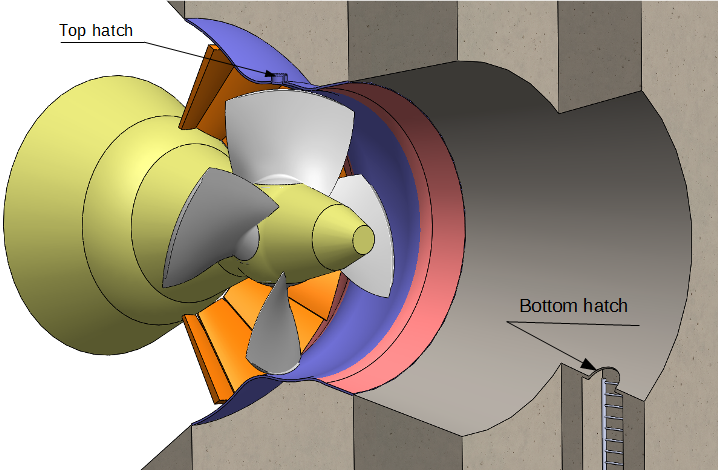
\includegraphics[width=\columnwidth]{figs/problem/ambiente_3d.PNG} 
	\caption{Jirau's hydropower turbine in a 3D CAD model.}
	\label{fig::ambiente3d}
\end{figure}

\end{comment}